Riportiamo adesso i risultati ottenuti con la tecnica di codifica d'immagine basata su DCT implementata. In Figura \ref{fig:original} è stata riportata l'immagine originale scelta per testare la codifica.
\begin{figure}[H]
    \centering
    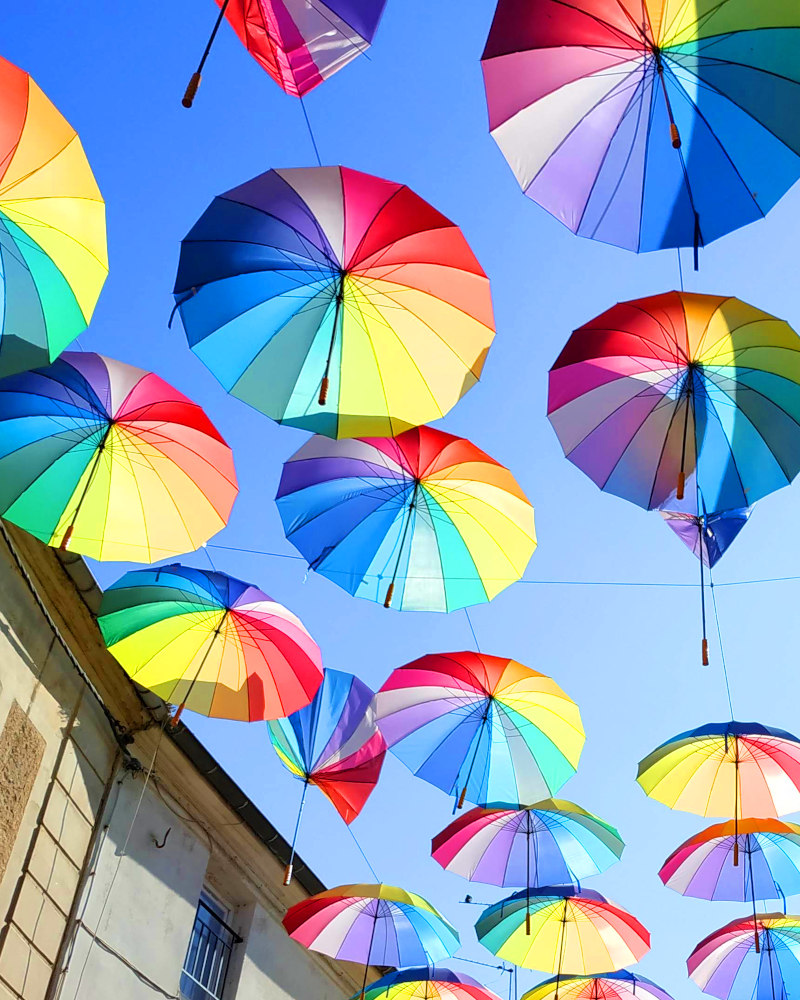
\includegraphics[width=0.65\linewidth]{Original.png}
    \caption{Immagine originale}
    \label{fig:original}
\end{figure}
Dapprima abbiamo tracciato i grafici del PSNR in funzione di $R$ per $N=8,16,64$, facendo variare il parametro $R$ da 10 a 100 in modo lineare a passi di 0.1 in modo da poter apprezzare al meglio l'andamento del grafico. Riportiamo quindi nelle Figure \ref{fig:ris8},\ref{fig:ris16} e \ref{fig:ris64} i grafici.
\begin{figure}[H]
    \centering
    \begin{minipage}{.5\textwidth}
        \centering
	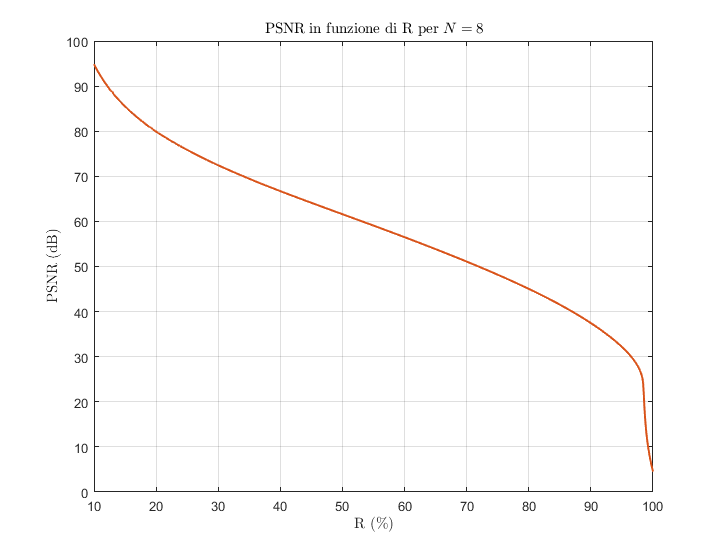
\includegraphics[width=\linewidth]{RIS_N8.png}
	\caption{$N=8$}
	\label{fig:ris8}
    \end{minipage}%
    \begin{minipage}{.5\textwidth}
        \centering
	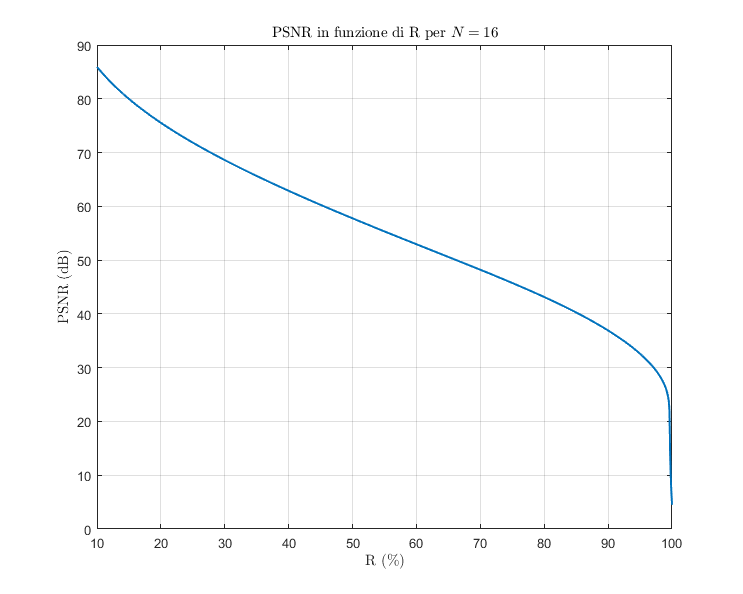
\includegraphics[width=\linewidth]{RIS_N16.png}
	\caption{$N=16$}
	\label{fig:ris16}
    \end{minipage}
\end{figure}
\begin{figure}[H]
	\centering
	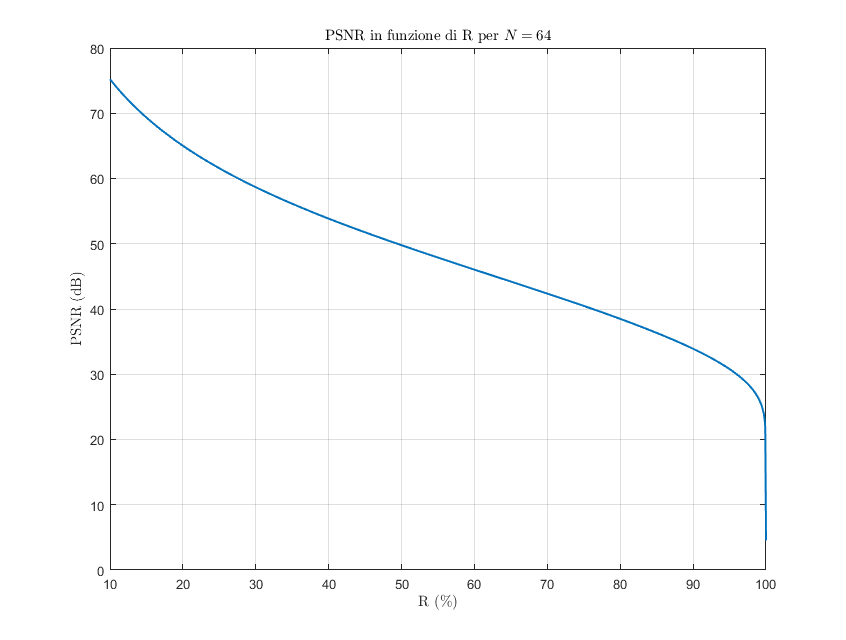
\includegraphics[width=0.75\linewidth]{RIS_N64.png}
	\caption{$N=64$}
	\label{fig:ris64}
\end{figure}
Si è voluto aumentare la "risoluzione" di $R$, rispetto alla consegna, per permettere di vedere il reale andamento del PSNR in funzione di $R$. Viene riportato in Figura \ref{fig:ris} l'andamento del grafico nel caso in cui il parametro $R$ viene fatto variare a passi di 10.
\begin{figure}[H]
	\centering
	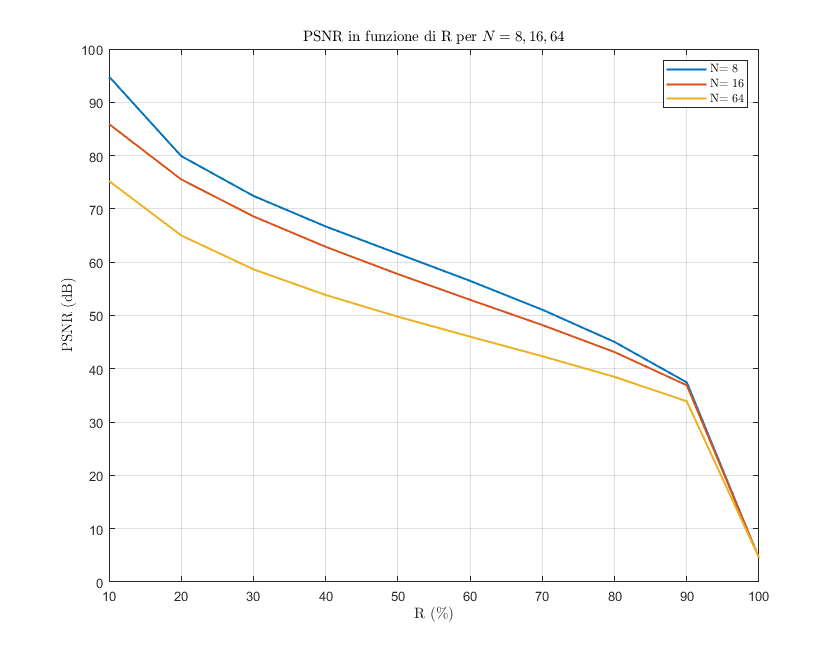
\includegraphics[width=0.7\linewidth]{RIS_TOT.png}
	\caption{Andamento del PSNR per $N=8,16,64$ con passo di $R$ a 10.}
	\label{fig:ris}
\end{figure}
Si osserva che all'aumentare della dimensione dei blocchi la compressione lavora meglio. Questo è dovuto al fatto che con blocchi più grandi è possibile raggruppare più informazioni spaziali in un unico blocco, sono meno sensibili alle variazioni locali dell'immagine, aumentando l'efficacia della codifica DCT. Si nota che per tutti i valori di $N$, il PSNR si riduce rapidamente per valori di $R$ superiori al 90\%\\\\
Si vuole sottolineare infine che il tempo computazionale aumenta sensibilmente diminuendo la dimensione del blocco.
\section{Risultati: immagini codificate}
Infine, riportiamo alcune immagini ricavate dalla nostra codifica, avendo impostato il fattore di compressione $R=98\%$ ad un valore abbastanza elevati per poter apprezzare come l'immagine si degrada a seguito della compressione.\\\\
Si può notare come la qualità dell'immagine compressa peggiora gradualmente all'aumentare della percentuale di coefficienti DCT posti a zero, con una perdita di dettagli e una comparsa di artefatti visibili in alcune zone dell'immagine. Tuttavia, anche quando viene impostata una percentuale elevata $(R>95\%)$, l'immagine compressa rimane abbastanza riconoscibile. Una compressione troppo aggressiva può causare una perdita di informazioni.
\begin{figure}[H]
    \centering
    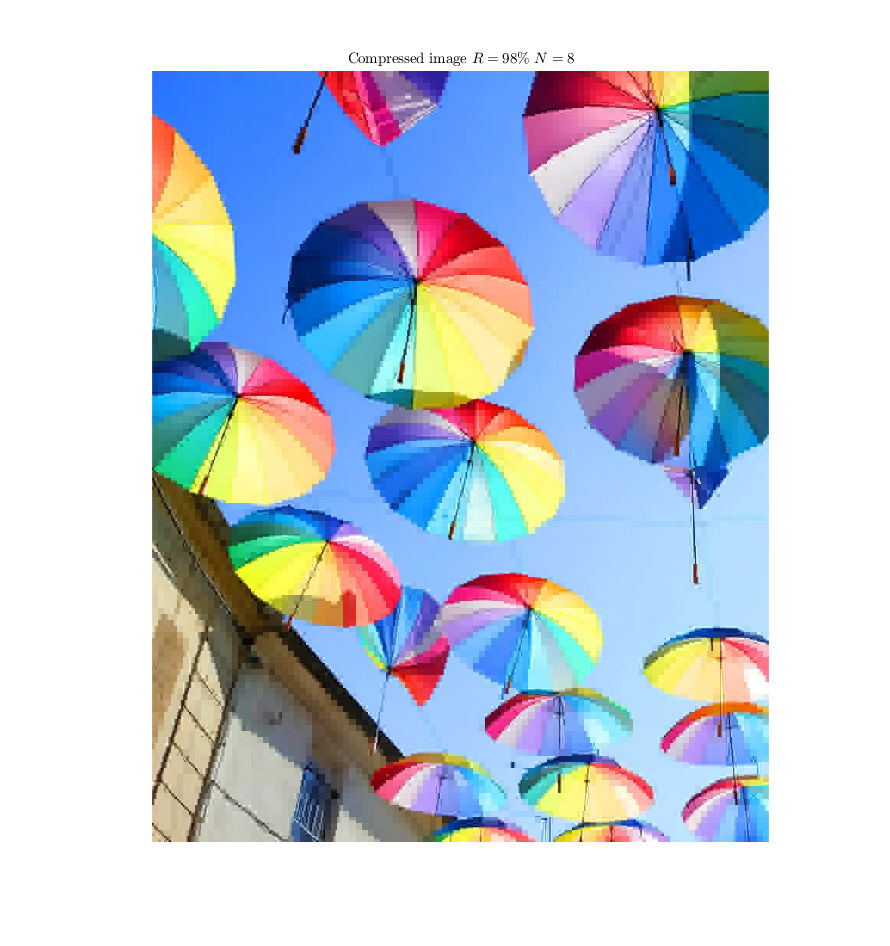
\includegraphics[width=\linewidth]{RIS_N8_R98.png}
    \caption{$N=8,R=98\%,PSNR=26.5859$}
    \label{fig:RIS_N8_R98}
\end{figure}
\begin{figure}[H]
    \centering
    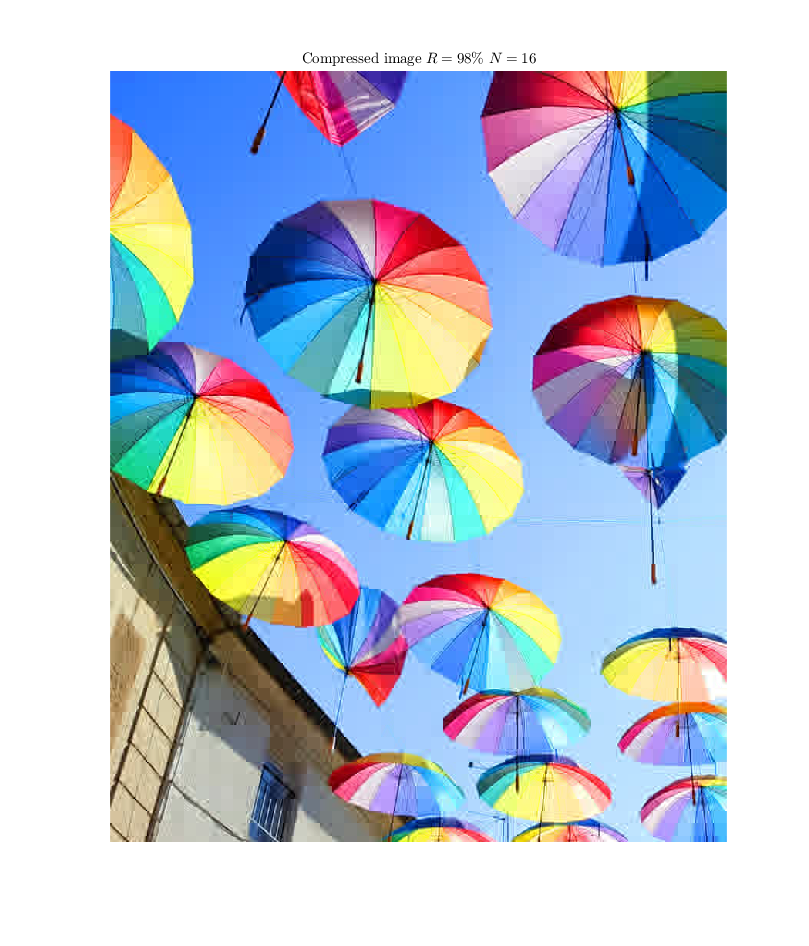
\includegraphics[width=\linewidth]{RIS_N16_R98.png}
    \caption{$N=16,R=98\%,PSNR=28.6002$}
    \label{fig:RIS_N16_R98}
\end{figure}
\begin{figure}[H]
    \centering
    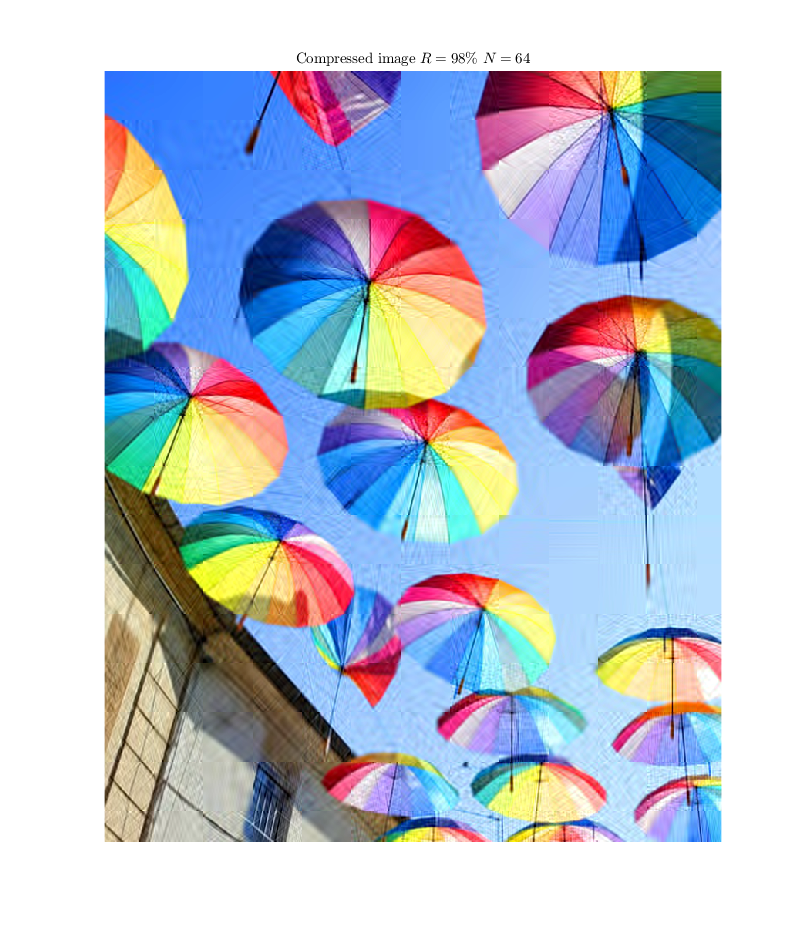
\includegraphics[width=\linewidth]{RIS_N64_R98.png}
    \caption{$N=64,R=98\%,PSNR=27.8918$}
    \label{fig:RIS_N64_R98}
\end{figure}